\chapter{Sparse Solutions of Underdetermined Systems}
\label{sparsity_background}
The method of least squares has been used for fitting models to data since Gauss invented the normal distribution and used it to predict the orbits of celestial bodies \autocite{Sti81}. With the law of large numbers ensuring that measurements often have Gaussian error, least squares serves its role well when no other prior information can be employed. This chapter is about the case when that isn't true, when we know something about the form of the solution itself: it is sparse. Images and audio are sparse; radar scenes are sparse; the brain uses sparsity to make sense of the world. Whenever something looks complex but is actually simple in the right form, that's sparsity. Across many applications, sparsity serves as a useful representation of prior knowledge.

The use of sparsity for inversion or fitting falls under a number of umbrella terms: compressed sensing, sparse approximation, low-rank decomposition, $l_1$-regularization, and many similar variants. Each of these means something slightly different, but the machinery behind them is the same. In all cases, a simple or sparse representation is sought for some data, and the key to getting it is a nonlinear method. The solution methods are more diverse than even the number of applications for them, and the list continues to grow. For our purposes, we will focus on the theory of compressed sensing because it provides good guidance for what kind of approaches will work best. We will also focus on solution methods based on convex optimization and particularly the prox operator, since these are easy to understand, flexible, have good theoretical underpinnings, and perform well in practice \autocite{PB13}. However, this choice is still somewhat arbitrary; the approach is the important part, and not so much the particular methods used.

\section{Underdetermined Systems of Equation}
\label{underdetermined_systems}
When performing model inversion, a common challenge is solving an underdetermined system of equations. In this situation, one has a matrix/vector equation such as
\begin{equation}
 y = Ax,
\end{equation}
where $y$ is a vector of length $M$ representing measurements, $A$ is a matrix that encompasses the mathematical model of the system, and $x$ is a vector of length $N$ giving unknown parameters. The equation is underdetermined because there are fewer measurements in $y$ than unknowns in $x$, so there are an infinite number of $x$ vectors that satisfy the equation. This situation can arise in many ways, but in general we can think of the underdetermined system as representing the decomposition of a signal $y$ using an overcomplete dictionary. The columns of the matrix $A$, denoted $a_n$, are the atoms of the dictionary, and the entries of $x$ are the coefficients corresponding to those atoms:
\begin{equation}
 y = \sum_{n=0}^{N-1} x[n] a_n.
\end{equation}
Since $M < N$, the dictionary atoms cannot form an orthogonal set, and there are many ways to form the decomposition \autocite{Mal08}. "Solving" the underdetermined system involves finding a preferable decomposition, one that at least has the qualities of the original measurement-generating solution when they are not the same.

\subsection{Least Norm Solution}
A common and linear solution method to an underdetermined system of equations is to take a least norm approach. Of the infinite number of solutions, it is simple to find the one with the smallest $l_2$-norm by performing the optimization
\begin{equation*}\tag{$\text{P}_\text{2}$}
 \begin{matrix*}[l]
  \underset{x}{\mathrm{minimize}} & \norm{2}{x}\\
  \text{subject to} & y = Ax,
 \end{matrix*}
\end{equation*}
where $\norm{2}{x} = \sum_k \abs{x[k]}^2$ denotes the $l_2$-norm. When $A$ is full rank (none of the measurements are redundant), $AA^*$ is invertible and the solution to the least norm problem is
\begin{equation}\label{eq:least_norm_solution}
 x_* = A^*(AA^*)^{-1}y.
\end{equation}
For situations when the measurements are noisy, one can turn to the related $l_2$-regularized least squares problem, also known as Tikhonov regularization:
\begin{equation*}\tag{$\text{P}_{\text{2}\lambda}$}
 \underset{x}{\mathrm{minimize}} \quad \norm{2}{y - Ax} + \lambda\norm{2}{x},
\end{equation*}
where $\lambda$ is the regularization parameter. This problem is solved by calculating 
\begin{equation}
 x_* = (A^*A + \lambda I)^{-1} A^* y,
\end{equation}
where $I$ is the identity matrix. As $\lambda \rightarrow 0$, the solution to $l_2$-regularized least squares converges to the least norm solution. Since these solutions are the result of basic matrix operations and are therefore linear, they are often favored for their ease of computation \autocite[Lecture 8]{Boy08}.

\subsection{Sparsest Solution}
Motivated by the inherent simplicity of answers to many practical problems, another approach to selecting a particular solution of an underdetermined system is to choose the sparsest solution. This problem can be written using the $l_0$ pseudo-norm, which is just the count of the number of nonzero entries in a vector:
\begin{equation}
 \norm{0}{x} = \#\set{k : x[k] \ne 0}.
\end{equation}
With this notation, the sparsest solution is found by the optimization problem
\begin{equation*}\tag{$\text{P}_\text{0}$}
 \begin{matrix*}[l]
  \underset{x}{\mathrm{minimize}} & \norm{0}{x}\\
  \text{subject to} & y = Ax.
 \end{matrix*}
\end{equation*}
Unfortunately, this problem is NP-hard in general \autocite{Nat95}, requiring combinatorial optimization to solve. Essentially, one has to check each sparsity pattern (location of zeros/nonzeros) for a solution until the sparsest one is found.

Fortunately, the convex relaxation of this problem, which is easy to solve, provides the sparsest solution in most cases. Instead of minimizing the $l_0$ pseudo-norm, one minimizes the $l_1$-norm:
\begin{equation*}\tag{$\text{P}_\text{1}$}\label{eq:l1min}
 \begin{matrix*}[l]
  \underset{x}{\mathrm{minimize}} & \norm{1}{x}\\
  \text{subject to} & y = Ax,
 \end{matrix*}
\end{equation*}
where $\norm{1}{x} = \sum_k \abs{x[k]}$ denotes the $l_1$-norm. Then for the overwhelming majority of matrices $A$ with columns normalized to one, there is a constant $\rho(M, N) > 0$ such that if $x_0$ is a solution to $y=Ax_0$ with at most $\rho M$ nonzeros, that solution is both the sparsest possible solution and the minimal $l_1$-norm solution \autocite{Don06}. In other words, whenever there is a sufficiently sparse solution, $l_1$ minimization will find it. The proof by \textcite{Don06} does not provide a practically useful formula for the breakdown point $\rho$, but it does provide motivation for why an equivalence of this kind must exist. It is easy to see how the $l_1$-norm promotes sparse solutions by equally penalizing both large and small nonzero values of $x$; equivalence comes from the rarity of truly sparse $x$ that actually solve the underdetermined system, causing $l_1$-minimization to pick out the true solution due to lack of other possibilities.

\section{Compressed Sensing}
\label{compressed_sensing}
Compressed sensing \autocite{Don06a, CW08} expands on the theory for solving underdetermined systems of equations when the solution is known to be sparse. It provides guarantees for recovering the true solution to within noise bounds provided that the measurements are "incoherent" and that their number is on the order of the solution sparsity. In essence, one only needs to measure at the information rate (sparsity) of the solution rather than fully sample the entire space of solutions. Not only that, but these optimal non-adaptive measurements, pre-determined and embodied in a measurement matrix, are known to perform nearly as well as the best adaptive measurements \autocite{Don06a}. The key is sparsity, which acts as the prior information that enables narrowing in on the one true answer out of the infinite potential answers.

\subsection{Conditions}
The main requirement for invoking the theory of compressed sensing is that the sought signal is sparse, or at least well-approximated by a sparse representation. In terms of a specified dictionary, sparsity requires that the signal be well-represented by a relatively small number of coefficients corresponding to the dictionary atoms. A signal might not be sparse in its natural representation, but that does not mean that it is not sparse in some other representation. Images are generally not sparse when specified by individual pixel values, but they are almost always sparse in a Fourier or wavelet dictionary. The only instance where this is not true is for images with high entropy; they are random and have no structure \autocite{Mal08}. Even if a signal $x$ is not exactly sparse, we say it has an $S$-sparse approximation if $\norm{2}{x - x_S}$ is small, where $x_S$ is the vector of coefficients $x[n]$ with all but the largest $S$ entries set to zero. As the success of lossy compression schemes demonstrate, many signals of interest satisfy at least this compressibility condition.

Measurement incoherence is the second condition for applying the theory of compressed sensing \autocite{CW08}. Consider the simplest case of a 1-sparse signal $x_1$ measured as $y=Ax_1$, with the number of measurements $M$ much less than the dimension of the signal $N$. At least one of the measurements must include a contribution from the nonzero entry of $x_1$ or else recovery from $y$ is impossible. Since we don't know \emph{a priori} which element is the nonzero one and because $M \ll N$, the only way to achieve a high probability of recovery is to have measurements that individually span a large portion of the unknown signal space. Each measurement must be global in some sense, embodying most of the unknown coefficients. This concept is known as measurement incoherence: none of the measurements are very concentrated (coherent) in the unknown space.

In the mathematical theory, incoherence can be guaranteed by a number of different but related conditions. Often it is theoretically convenient to allow the measurements to be random. For an orthogonal set of possible measurements given by the matrix $U$ with scaling $U^*U = N \cdot I$, we can let the measurement matrix $A$ be a random subset of $M$ rows of $U$. The coherence $\mu(U)$ of the measurement set is then defined as
\begin{equation}
 \mu(U) = \max_{k,n} \; \abs[\big]{U[k,n]}^2,
\end{equation}
and it varies in value from a minimum of $1$ to a maximum of $N$ \autocite{CR07}. Thus, the measurements are incoherent under this framework when the set from which they are drawn has $\mu(U)$ close to $1$. The coherence parameter can also be defined for a wider class of probabilistic measurement ensembles, including Gaussian and binary random measurements, as shown by \textcite{CP11}.

Deterministic measurements can have their incoherence measured by the restricted isometry property (RIP) introduced by \textcite{CT06} and expanded upon in \textcite{CRT06}. Let $A_T$ with $T \subset \set{0, \dotsc, N-1}$ denote a subset of the columns of the measurement matrix $A$. Then the $S$-restricted isometry constant $\delta_S$ of $A$ is defined as the smallest number such that
\begin{equation}
 (1 - \delta_S)\norm{2}{x_S}^2 \le \norm{2}{A_T x_S}^2 \le (1 + \delta_S)\norm{2}{x_S}^2
\end{equation}
for all $S$-sparse vectors $x_S$ and all subsets $T$ with $\abs{T} \le S$. The restricted isometry property is satisfied and sufficient incoherence assured for a solution with sparsity $S$ when $\delta_{2S}$ is small enough. This condition ensures that the measurements preserve the distance between any two $S$-sparse solutions, guaranteeing that any $S$-sparse answer is unique.

\subsection{Theoretical Bounds}
If the signal is compressible and incoherent sampling is performed, then essentially we know that each measurement contains a contribution from each of the $S$ coefficients. Intuitively, we might then expect to be able to reconstruct the signal from about $S$ measurements. This idea is made concrete with the incoherent sampling theorem presented below for reconstruction via the $l_1$-minimization problem \eqref{eq:l1min}. No matter the specific setting, the principle of this theorem remains the same: if the sampling is incoherent and we solve an appropriate convex optimization problem, we can reconstruct a signal to within noise and $S$-sparse approximation errors by using on the order of $S\log{N}$ measurements.

In the case where we know the coherence $\mu(U)$ of the measurements, the incoherent sampling theorem requires a number of measurements $M$ that meets the condition $M \ge C \cdot \mu(U) \cdot S \cdot \log{N}$ for a sparsity level $S$ and constant $C$. In the case where measurement incoherence is guaranteed in terms of the restricted isometry property, we require $\delta_{2S} < \sqrt{2} - 1$ for a specified sparsity level $S$. For random Gaussian or binary matrices, the RIP requirement on $\delta_{2S}$ is satisfied with overwhelming probability when $M \ge C \cdot S \cdot \log{(N/S)}$. In either case, the recovery bound has the same form. Denoting the result of the $l_1$-minimization problem as $x_*$, the true solution as $x$, and the best $S$-sparse approximation of $x$ as $x_S$, we have
\begin{equation}
 \norm{2}{x_* - x} \le C_0 \norm{2}{x - x_S},
\end{equation}
where $C_0$ is a small known constant. The coherence parameter result is due to \textcite{CP11}, while the RIP result is due to \textcite{Can08}. Both articles specify values for the constants $C$ and $C_0$, but they are believed to be sub-optimal in general, hence the imprecision. If $x$ is exactly $S$-sparse, this says that $l_1$-minimization finds the exact sparse solution. When $x$ is not $S$-sparse, the $l_1$ solution is nearly as close to the true solution as the best $S$-sparse approximation. In other words, the reconstruction is almost as good as the best possible given by a so-called oracle; we could hardly do better if we knew the locations of the $S$ most significant elements of $x$ ahead of time.

The incoherent sampling theorem can also be extended to cases with measurement error. Suppose that the measurements are now given by
\begin{equation}
 y = Ax + \eta,
\end{equation}
where $\eta$ is an unknown noise term. In this setting, we are interested in the solution to the basis pursuit with denoising problem:
\begin{equation*}\tag{$\text{P}_{\text{1}\epsilon}$}\label{eq:BPDN}
 \begin{matrix*}[l]
  \underset{x}{\mathrm{minimize}} & \norm{1}{x}\\
  \text{subject to} & \norm{2}{y - Ax} \le \epsilon,
 \end{matrix*}
\end{equation*}
where $\epsilon$ is a chosen noise bound. Then under the same restricted isometry condition $\delta_{2S} < \sqrt{2} - 1$ as before, the solution $x_*$ to \eqref{eq:BPDN} satisfies
\begin{equation}
 \norm{2}{x_* - x} \le C_0 \norm{2}{x - x_S} + C_1 \epsilon,
\end{equation}
where $C_0$ and $C_1$ are small known constants with similar interpretations as before \autocite{Can08}. This remarkable result shows that $l_1$-recovery is robust to noise; the error in the answer is still bounded only by the approximation error and the noise level. A similar result is given by \textcite{CP11} for the case when only the coherence $\mu(U)$ is known, although the noise term is handled a little differently.

\subsection{Recovery Phase Transition}
It may seem unlikely that adding noise to the problem does not dramatically worsen recovery of the true solution, but amazingly this has proven to be true in a growing list of cases. \textcite{DMM11} completely characterize the phase transition from failed recovery to successful solution over the space of $(\delta, \rho)$ with $\delta = M/N$ and $\rho = S/M$ for measurement matrices $A$ whose entries are i.i.d.\ Gaussian. For a given undersampling ratio $\delta$, recovery is successful with overwhelming probability for $\rho$ below the curve $\rho_\text{MSE}(\delta)$, and it fails with overwhelming probability otherwise. The phase transition curve is shown in Figure \ref{fig:l1_phase_transition}.
\begin{figure}[tpb]
 \centering
 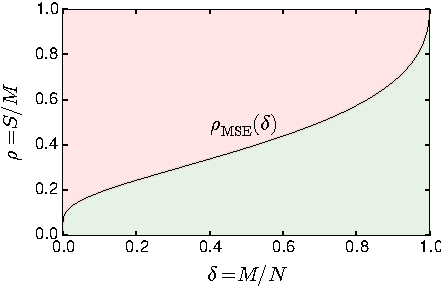
\includegraphics{l1_phase_transition}
 \caption[Phase transition for recovery of sparse solution]{\emph{Phase transition for recovery of sparse solution.} For noisy measurements $y \in \field{R}^M$ given by $y=Ax + \eta$, recovery of $S$-sparse $x \in \field{R}^N$ by is successful (mean square error is bounded) when $\rho = S/M$ is below the curve $\rho_\text{MSE}(\delta)$ shown above with $\delta = M/N$. The result holds for many types of measurement matrices $A$ and nonlinear recovery algorithms, particularly $l_1$ minimization.}
 \label{fig:l1_phase_transition}
\end{figure}%
For these results, successful recovery means that the measurement error is bounded for the worst-case noise and sparsity distributions, while failure means that the error is unbounded. The theoretical results are for the limit as $M$, $N$, and $S$ tend to infinity with fixed $(\delta, \rho)$, but simulations have shown that the transition holds for finite setups.

It must be emphasized that this phase transition represents the behavior of the \emph{optimal} recovery algorithm when faced with the parameters of the problem. The key to the success of compressed sensing is that $l_1$ minimization \emph{is} an optimal recovery algorithm; it achieves this performance with appropriate choice of the noise parameter \autocite{DT09, DMM11}. Furthermore, the optimal performance has been shown to extend empirically to other measurement ensembles \autocite{DT10, MJG+13} and theoretically to other optimization algorithms \autocite{DJM13}. Research in this area is ongoing and advancing rapidly, and it is expected that the recovery bounds and phase transition results apply to a wider class of measurement ensembles and recovery algorithms than have so far been proven. Along this line, \textcite{Str12} gives an overview of the open problems that remain to be solved.

\section{Convex Optimization}
\label{convex_optimization}
Sparse solutions to an underdetermined system of equations can be sought with a bevy of different methods. Some of these are greedy algorithms like OMP (orthogonal matching pursuit) \autocite{TG07}, some are based on statistics like AMP (approximate message passing) \autocite{DMM09}, and most are variants that improve on a basic method in some way. Of particular note are the many methods that involve a common but not universal theme: convex optimization, specifically involving minimization of the $l_1$-norm. Our focus is on methods of this type because they are easy to understand and the theory is well-established. The base case is an optimization problem known as $l_1$-regularized least squares:
\begin{equation*}\tag{$\text{P}_{\text{1}\lambda}$} \label{eq:l1rls}
 \underset{x}{\mathrm{minimize}} \quad \frac{1}{2}\norm{2}{Ax - b}^2 + \lambda\norm{1}{x}.
\end{equation*}
This problem is equivalent to basis pursuit with denoising \eqref{eq:BPDN} for a proper choice of the regularization parameter $\lambda$, but its form is more convenient for many algorithms.

\subsection{First-order Methods}
Before discussing $l_1$-regularized least squares specifically, we restrict our attention to a particular class of optimization algorithms: first-order methods. For the types of problems that we are interested in, explicit representations of the measurement matrix $A$ are not useful. The typical matrix is large and has additional structure that makes applying it via matrix multiplication inefficient. When $A$ represents convolution, a Fourier transform, or other efficient transforms as is often the case, it is much faster to compute its result using the transform operation directly. First-order optimization algorithms are interesting because they do not require using an explicit matrix representation for $A$ and $A^*$; they only require the ability to evaluate the $A$ and $A^*$ operations, which we can do efficiently even for large problem dimensions.

The most natural first-order method for minimizing a differentiable convex function $G(x)$ is gradient descent. Starting at a point $x^0$, gradient descent iteratively steps in the direction of the negative of the gradient $\grad_{G}(x) = \nabla G(x)$ until the minimum is reached.
\begin{algorithm}[H]
 \caption{Gradient Descent \autocite{Boy04}}
 \begin{algorithmic}
  \GIVEN a starting point $x^0$
  \REPEAT
  \STATE $x^{k+1} \coloneqq x^{k} - \mu \grad_{G}(x^{k})$ \COMMENT{step size $\mu$ chosen by line search}
  \UNTIL{stopping criterion is satisfied}
 \end{algorithmic}
\end{algorithm}\noindent
Gradient descent is guaranteed to converge to a minimum-value solution for smooth, convex $G(x)$ provided that the step size is chosen appropriately. This is typically done with a backtracking line search as detailed by \textcite{Boy04}. For the function $G(x) = \frac{1}{2}\norm{2}{Ax - b}^2$, the gradient is $\grad_{G}(x) = A^*(Ax - b)$. Thus in order to iteratively find the least squares solution to $Ax=b$ using gradient descent, we only need to be able to evaluate $A$ and $A^*$.

Of course, the function we want to minimize to be able to solve the $l_1$-regularized least squares problem is not differentiable, so gradient descent is not directly applicable. For non-smooth functions $F(x)$ like the $l_1$-norm, an attractive alternative to the gradient is the \emph{proximal operator}:
\begin{equation}
 \prox_{\mu F} (v) = \argmin_{x} \; \paren*{F(x) + \frac{1}{2\mu} \norm{2}{x - v}^2},
\end{equation}
where $\mu$ is a scaling factor that can be likened to a step size. The prox operator adds an $l_2$-smoothing term to a non-smooth function and outputs the vector $x$ which gives the minimum of the composite function. Using the prox operator as an iterative step in a similar manner to the gradient leads to an algorithm for minimizing non-smooth $F(x)$: the proximal point method.
\begin{algorithm}[H]
 \caption{Proximal Point \autocite{PB13}}
 \begin{algorithmic}
  \GIVEN a starting point $x^0$
  \REPEAT
  \STATE $x^{k+1} \coloneqq \prox_{\mu F}(x^{k})$ \COMMENT{scaling $\mu$ chosen by line search}
  \UNTIL{stopping criterion is satisfied}
 \end{algorithmic}
\end{algorithm}\noindent
Note that as the iterates $x^{k}$ approach the minimum $x_*$, the smoothing term goes to zero and the minimum of $F(x)$ is reached.

\subsection{Prox Operator Examples}
For many interesting functions $F(x)$, the prox operator is surprisingly easy to solve. The prox operator of the $l_1$-norm will obviously be useful, and fortunately it has a closed form solution known as soft thresholding:
\begin{equation}
 \prox_{\tau \norm{1}{x}} (v) = \soft_{\tau}(v)[k] =
    \begin{cases}
      \paren*{1 - \frac{\tau}{\abs{v[k]}}} v[k], & \abs[\big]{v[k]} > \tau\\
      0, & \abs[\big]{v[k]} \le \tau.
     \end{cases}
\end{equation}
Soft thresholding operates element-wise on a vector $v$, setting all of the elements with magnitude less than the threshold $\tau$ to zero and shrinking all other elements toward zero by $\tau$. A graphical depiction of scalar soft thresholding is given in Figure \ref{fig:soft_thresholding}.
\begin{figure}[tpb]
 \centering
 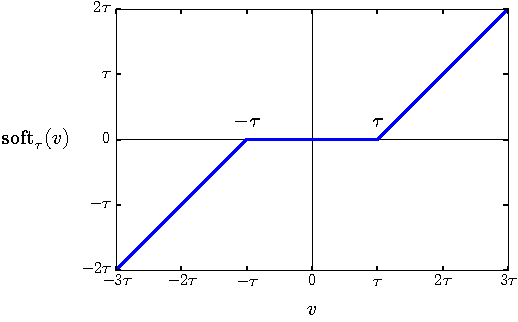
\includegraphics{soft_thresholding_function}
 \caption[Soft thresholding function]{\emph{Soft thresholding function.} The real scalar soft thresholding function evaluates to zero when the magnitude of the input is below the threshold $\tau$, and it returns a shrunken value of the input otherwise.}
 \label{fig:soft_thresholding}
\end{figure}%

The $l_2$-norm, though smooth, also has a closed form prox operator. For $F(x) = \norm{2}{x}$, the prox operator is the block soft thresholding operator,
\begin{equation}
 \prox_{\tau \norm{2}{x}} (v) = \bsoft_{\tau}(v) =
    \begin{cases}
      \paren*{1 - \frac{\tau}{\norm{2}{v}}} v, & \norm{2}{v} > \tau\\
      0, & \norm{2}{v} \le \tau.
     \end{cases}
\end{equation}
Block soft thresholding operates on the entire vector $v$, setting it to zero if its norm is less than the threshold $\tau$ and shrinking its norm to $\norm{2}{v} - \tau$ otherwise. The squared $l_2$-norm $F(x) = \frac{1}{2}\norm{2}{x}^2$ has a different prox operator called the shrinkage function:
\begin{equation}
 \prox_{\frac{\tau}{2}\norm{2}{x}^2} (v) = \shrink_{\tau}(v) = \frac{v}{1 + \tau}.
\end{equation}
In contrast to soft thresholding, the shrinkage function shrinks all of the vectors' entries by a fixed fraction defined by the scale factor $\tau$, penalizing the largest entries the most.

When the non-smooth function is the indicator $I_{\mathcal{C}}(x)$ for a closed nonempty convex set $\mathcal{C}$, which is defined as
\begin{equation}
 I_{\mathcal{C}}(x) = \begin{cases}
                       0, & x \in \mathcal{C}\\
                       +\infty, & x \notin \mathcal{C},
                      \end{cases}
\end{equation}
the prox operator acts as Euclidean projection onto $\mathcal{C}$:
\begin{equation}
 \prox_{I_{\mathcal{C}}} (v) = \argmin_{x} \; \paren*{I_{\mathcal{C}}(x) + \frac{1}{2} \norm{2}{x - v}^2} = \argmin_{x \in \mathcal{C}} \; \norm{2}{x - v} = \Pi_{\mathcal{C}}(v).
\end{equation}
When viewed in this way, prox operators can be seen as generalized projections. In the case of the $l_1$-norm, soft thresholding "projects" onto a sparse space enforced by the $l_1$-norm by setting small elements to zero. Practically, indicator functions are useful for enforcing constraints in optimization problems. By adding an appropriate indicator function to the objective, solutions can be required to lie in the corresponding convex set. For example, if a solution to an underdetermined system is known to have a particular sparsity pattern, the indicator function for the locations of the zeros can be added to a least squares objective to solve for the closest solution with that sparsity pattern.

\subsection{Proximal Gradient}
With the necessary operators in place, we finally return to the problem of $l_1$-regularized least squares \eqref{eq:l1rls}. This is a problem of the form
\begin{equation}
 \underset{x}{\mathrm{minimize}} \quad F(x) + G(Ax - b),
\end{equation}
where $F(x)$ is (possibly non-differentiable) function with a known prox operator $\prox_{F} (v)$, $A$ is a linear operator, $b$ is a vector constant, and $G(z)$ is a differentiable function so that the gradient of the second term is $A^* \grad_{G}(Ax - b)$. With the split smooth and non-smooth objective, we can imagine a two-step iteration stage that first steps in the gradient direction of the smooth term and then evaluates the prox operator of the non-smooth term. This leads to an optimization algorithm known as the proximal gradient method.
\begin{algorithm}[h]
 \caption{Proximal Gradient \autocite{PB13}}
 \begin{algorithmic}
  \GIVEN a starting point $x^0$, a step size $0 < \mu \le 2/L$
  \REPEAT
  \STATE $z^{k+1} \coloneqq x^k - \mu \, A^* \grad_{G}(Ax^k - b)$
  \STATE $x^{k+1} \coloneqq \prox_{\mu F}(z^{k+1})$
  \UNTIL{stopping criterion is satisfied}
 \end{algorithmic}
\end{algorithm}\\
Stopping criteria for the algorithm vary, but we will choose one based on the residual of the optimality condition $0 \in \partial F(x_*) + \nabla_x G(Ax_* - b)$. This residual for the iterate $x^{k+1}$ is given by
\begin{equation}
 r^{k+1} = \frac{1}{\mu}\paren*{x^k - x^{k+1}} + A^*\paren*{\grad_G(Ax^{k+1} - b) - \grad_G(Ax^k - b)}.
\end{equation}
The algorithm is said to have converged if $\norm{2}{r^{k+1}}$ is small, less than a tolerance threshold. The basic proximal gradient method also uses a fixed step size $\mu > 0$, and to guarantee convergence it must satisfy $\mu \le 2/L$ where $L$ is the global Lipschitz constant of the gradient of $G(Ax - b)$. For all $x$, $\tilde{x}$ in the domain of $\nabla_x G$, the gradient is globally Lipschitz continuous if
\begin{equation}
 \norm{2}{\nabla_x G(Ax - b) - \nabla_x G(A\tilde{x} - b)} \le L \norm{2}{x - \tilde{x}}.
\end{equation}

One interpretation of the proximal gradient method is as a majorization-minimization algorithm. At every step, the algorithm majorizes (upper bounds) the objective and then minimizes the majorization. In this case, the majorization involves taking a first-order approximation of the smooth portion of the objective and adding a trust region penalty:
\begin{equation}
 G_{\mu}(x, \tilde{x}) = G(\tilde{x}) + \innerprod*{\nabla_x G(A\tilde{x} - b)}{x - \tilde{x}} + \frac{1}{2\mu}\norm{2}{x - \tilde{x}}^2.
\end{equation}
Then for $\mu \le 1/L$, we have the majorization
\begin{equation}
 F(x) + G(Ax - b) \le F(x) + G(x^{k}) + \innerprod*{\nabla_x G(Ax^{k} - b)}{x - x^{k}} + \frac{1}{2\mu}\norm{2}{x - x^{k}}^2
\end{equation}
about the point $x^{k}$. Minimizing the majorization is just a simple call to the prox operator of $F$:
\begin{align}
 x^{k+1} &= \argmin_{x} \; \paren*{F(x) + G(x^{k}) + \innerprod*{\nabla_x G(Ax^{k} - b)}{x - x^{k}} + \frac{1}{2\mu}\norm{2}{x - x^{k}}^2}\nonumber\\
 &= \argmin_{x} \; \paren*{F(x) + \frac{1}{2\mu}\norm{2}{x - \paren*{x^{k} - \mu \, A^* \grad_G(Ax^k - b)}}}\nonumber\\
 &= \prox_{\mu F}\paren*{x^{k} - \mu \, A^* \grad_G(Ax^k - b)}.
\end{align}
This step is precisely the one taken in the proximal gradient method.

Proximal gradient applied to the $l_1$-regularized least squares problem has a special name: iterative soft thresholding. If we divide the objective as $F(x) = \lambda\norm{1}{x}$ and $G(z) = \frac{1}{2}\norm{2}{z}$, the proximal operator $\prox_{F}(x) = \soft_{\lambda}(x)$ is soft thresholding, the gradient $\grad_{G}(z) = z$ is the identity, and the method takes the explicit form given in Algorithm \ref{alg:ist}.
\begin{algorithm}[H]
 \caption{Iterative Soft Thresholding}
 \label{alg:ist}
 \begin{algorithmic}
  \GIVEN a starting point $x^0$, a step size $0 < \mu \le 2/\norm{2}{A}^2$
  \REPEAT
  \STATE $z^{k+1} \coloneqq x^k - \mu \, A^*(Ax^k - b)$
  \STATE $x^{k+1} \coloneqq \soft_{\mu \lambda}(z^{k+1})$
  \UNTIL{stopping criterion is satisfied}
 \end{algorithmic}
\end{algorithm}\noindent
Clearly the iterative soft thresholding method is aptly named. With the form of the gradient known, we also know that its Lipschitz constant $L$ is given by $\norm{2}{A}^2$, the squared induced $l_2$-norm of the matrix $A$. If $A$ is scaled so that its norm is unity, then the maximum fixed step size that guarantees convergence is $2$.

\subsection{Improvements on Proximal Gradient}
The proximal gradient method can be improved both theoretically and in practice through the use of an acceleration term and a variable step size. Acceleration of first-order methods is based on the work of \textcite{Nes83, Nes88} for smooth objectives, which was extended by \textcite{BT09, BT10} to the proximal gradient method. \textcite{Nes07} also adapted acceleration to the case of a composite objective, but that particular approach requires multiple evaluations of the prox operator per step. Acceleration works by adding an appropriate ratio of the prior iterate to the current iterate before executing the gradient and prox steps, thus this simple modification improves convergence without significantly increasing per-step computation. More recently, \textcite{OC13} found that an adaptive restart scheme for the acceleration term improves convergence in practice even more significantly. Applied to the $l_1$-regularized least squares problem, the accelerated method is known as FISTA, or the fast iterative soft thresholding algorithm \autocite{BT09}.

A variable step size is the other modification that practically improves performance. Though convergence is guaranteed by bounding the steps by the global Lipschitz constant, such steps can be too conservative when the gradient's curvature is locally variable. When this is the case, even a standard backtracking line search for the step size is not sufficient since it can only decrease the step size. Both \textcite{SGB11} and \textcite{BCG11}, apparently independently, suggested an expansive backtracking line search scheme to accommodate increasing the step size if warranted. With this scheme, the step size is increased by a constant factor after every iteration; convergence is assured by checking the majorization condition at the next iterate and backtracking on the step size by a constant factor if necessary. Though backtracking results in repeated application of $A$, $A^*$, and the gradient and prox operators, the typical net result is fewer computations and faster convergence. With both the acceleration and variable step size enhancements, we get a proximal gradient method that significantly improves upon the performance of the basic method. The accelerated proximal gradient method, with adaptive restart and adaptive step size, is detailed as Algorithm \ref{alg:accelproxgrad}.
\begin{algorithm}[tpb]
 \caption{Accelerated Proximal Gradient, with adaptive restart and adaptive step size}
 \label{alg:accelproxgrad}
 \begin{algorithmic}
  \GIVEN starting point $x^0$
  \GIVEN initial step size $\mu^0 > 0$, step expansion factor $\alpha > 1$, backtracking factor $0 < \beta < 1$
  \GIVEN tolerance $\epsilon > 0$
  \STATE $x^{-1}, w^0 \coloneqq x^0$
  \STATE $g^0 \coloneqq A^* \grad_{G}(Aw^0 - b)$

  \STATE $t^0 \coloneqq 1$
  \STATE $\mu^1 = \mu^0$
  \STATE $\gamma \coloneqq 1$
  
  \REPEAT
   \IF {$\innerprod*{w^k - x^k}{x^k - x^{k-1}} > 0$}
    \STATE $t^k \coloneqq 1$
   \ENDIF
   \REPEAT
    \STATE $t^{k+1} \coloneqq \paren*{1 + \sqrt{1 + 4\paren*{t^k}^2 \gamma}}/2$
    \STATE $\theta \coloneqq \paren*{t^k - 1}/t^{k+1}$
    \STATE $w^{k+1} \coloneqq x^k + \theta \paren*{x^k - x^{k+1}}$
    \STATE
    \STATE $g^{k+1} \coloneqq A^* \grad_{G}\paren*{Aw^{k+1} - b}$
    \STATE $x^{k+1} \coloneqq \prox_{\mu^{k+1} F}\paren*{w^{k+1} - \mu^{k+1} \, g^{k+1}}$
    \STATE
    \IF {$G(Ax^{k+1} - b) \le G(Aw^{k+1} - b) + \innerprod*{x^{k+1} - x^k}{g^{k+1}} + \frac{1}{2\mu^{k+1}}\norm{2}{x^{k+1} - w^{k+1}}^2$}
     \STATE \textbf{break}
    \ELSE
     \STATE $\mu^{k+1} \coloneqq \beta \mu^{k+1}$
     \STATE $\gamma \coloneqq \mu^{k} / \mu^{k+1}$
    \ENDIF
   \UNTIL
   \STATE $r^{k+1} \coloneqq \paren*{x^k - x^{k+1}}/\mu^{k+1} + g^{k+1} - g^k$
   \IF {$\norm{2}{r^{k+1}} \le \epsilon$}
    \STATE \textbf{break}
   \ENDIF
   \STATE $\mu^{k+1} \coloneqq \alpha \mu^{k+1}$
   \STATE $\gamma = \mu^k / \mu^{k+1}$
  \UNTIL
 \end{algorithmic}
\end{algorithm}%

\subsection{Related Prox Methods}
Naturally, there are other algorithms that solve the same (or a similar) split objective optimization problem and even make use of the prox operator. While proximal gradient requires part of the objective, $G(z)$, to be differentiable, these additional methods work in the more general case where only an easily-evaluated prox operator is required for each of the split-objective terms. Since this is a less-restrictive requirement, these methods are primarily of interest due to their broader applicability. Depending on the exact problem being solved, however, it is certainly possible for them to outperform even the accelerated proximal gradient method.

The alternating direction method of multipliers (ADMM) algorithm, also known as Douglas-Rachford splitting, solves the problem
\begin{equation}
 \underset{x}{\mathrm{minimize}} \quad F(x) + G(x)
\end{equation}
where both $F$ and $G$ have prox operators given by $\prox_{F}(x)$ and $\prox_{G}(x)$. Notice that this definition does not include the affine transformation $Ax - b$ as with the proximal gradient method. The ADMM algorithm is similar to proximal gradient in that it splits the iteration into two steps, first applying $\prox_{F}(x)$ and then applying $\prox_{G}(x)$ as detailed in Algorithm \ref{alg:admm}. Amazingly, the algorithm converges for any positive value of the penalty parameter $\rho$. ADMM can vary in its exact form depending on which order the prox operators are applied or, equivalently, by how the objective is split and assigned to the two functions, so care must be taken to choose the optimal formulation for a given problem. A detailed treatment of ADMM, including per-iteration adjustment of the penalty parameter to help improve convergence, is given by \textcite{BPC+11}.
\begin{algorithm}[tpb]
 \caption{Alternating Direction Method of Multipliers (ADMM)}
 \label{alg:admm}
 \begin{algorithmic}
  \GIVEN starting point $x^0$ with dual $y^0$, penalty parameter $\rho > 0$
  \STATE $u^0 \coloneqq \rho y^0$
  \STATE $z^0 \coloneqq \prox_{\rho G}\paren*{x^0 + u^0}$
  \REPEAT
   \STATE $x^{k+1} \coloneqq \prox_{\rho F}\paren*{z^k - u^k}$
   \STATE $z^{k+1} \coloneqq \prox_{\rho G}\paren*{x^{k+1} + u^k}$

   \STATE $r^{k+1} \coloneqq x^{k+1} - z^{k+1}$
   \STATE $s^{k+1} \coloneqq \paren*{z^k - z^{k+1}}/\rho$

   \STATE $u^{k+1} \coloneqq u^k + r^{k+1}$
  \UNTIL{$\norm{2}{r^{k+1}}$ and $\norm{2}{s^{k+1}}$ are small}
 \end{algorithmic}
\end{algorithm}%

Linearized ADMM, also called the Split Inexact Uzawa method \autocite{EZC10}, is a variant of ADMM that includes an affine transformation in the objective function with a matrix $A$ and vector $b$:
\begin{equation}
 \underset{x}{\mathrm{minimize}} \quad F(x) + G(Ax - b),
\end{equation}
where again $F$ and $G$ are not necessarily differentiable and have prox operators $\prox_{F}(x)$ and $\prox_{G}(z)$. It is not trivial to accommodate an affine transformation when evaluating the prox operator of most functions, so the explicit inclusion here is significant in practice and the reason linearized ADMM is often used over the original. Our version of linearized ADMM, given in Algorithm \ref{alg:admmlin}, is based on the one described by \textcite{PB13}. However, ours is unique because it includes not only a penalty adjustment scheme adapted from the ADMM method of \textcite{BPC+11} but also a novel expansive backtracking line search for the step size $\mu$. In fact, the interpretation of the $\mu$ parameter as a step size is unique, and doing so allows us to adapt the majorization condition and line search scheme used in the accelerated proximal gradient algorithm (Algorithm \ref{alg:accelproxgrad}) for use with linearized ADMM. We have not formally analyzed the convergence of linearized ADMM including these modifications or rigorously proved their benefits, but they do result in significant improvement in practice in a manner similar to the corresponding proximal gradient method schemes. As a point of reference, we have found that an expansion factor of $\alpha=1.25$, a backtracking factor of $\beta=0.5$, a maximum residual gap of $\gamma=10$, and a penalty factor of $\rho=1.5$ are the most effective parameters for a variety of problems.
\begin{algorithm}[tpb]
 \caption{Linearized ADMM}
 \label{alg:admmlin}
 \begin{algorithmic}
  \GIVEN starting point $x^0$ with dual $y^0$
  \GIVEN step size $\mu > 0$, step expansion factor $\alpha > 1$, backtracking factor $0 < \beta < 1$
  \GIVEN penalty parameter $\rho > 0$, maximum residual gap $\gamma > 1$, penalty factor $\tau > 1$
  \GIVEN penalty freezing index $k_{\rho_\text{max}}$
  \STATE $u^0 \coloneqq \rho y^0$
  \STATE $u^{-1} \coloneqq u^0$
  \REPEAT
   \REPEAT
    \STATE $x^{k+1} \coloneqq \prox_{\mu F}\paren*{x^k - \frac{\mu}{\rho} A^*\paren*{2u^k - u^{k-1}}}$
    \IF {$\mu \norm{2}{A\paren*{x^{k+1} - x^k}}^2 \le \rho \norm{2}{x^{k+1} - x^k}^2$}
     \STATE \textbf{break}
    \ELSE
     \STATE $\mu \coloneqq \beta \mu$
    \ENDIF
   \UNTIL
   \STATE $z^{k+1} \coloneqq \prox_{\rho G}\paren*{Ax^{k+1} - b + u^k}$

   \STATE $r^{k+1} \coloneqq Ax^{k+1} - b - z^{k+1}$

   \STATE $u^{k+1} \coloneqq u^k + r^{k+1}$
   
   \STATE $s^{k+1} \coloneqq A^*\paren*{u^{k+1} - u^k}/\rho + A^*\paren*{u^{k-1} - u^k}/\rho + \paren*{x^k - x^{k+1}}/\mu$
   
   \IF {$k < k_{\rho_\text{max}}$}
    \IF {$\norm{2}{r^{k+1}} > \gamma \norm{2}{s^{k+1}}$}
     \STATE $\rho = \rho/\tau$
     \STATE $u^{k+1} = u^{k+1}/\tau$
     \STATE $u^k = u^k/\tau$
    \ENDIF
    \IF {$\norm{2}{s^{k+1}} > \gamma \norm{2}{r^{k+1}}$}
     \STATE $\rho = \rho\tau$
     \STATE $u^{k+1} = u^{k+1}\tau$
     \STATE $u^k = u^k\tau$
    \ENDIF
   \ENDIF
   
   \IF {$\norm{2}{A\paren*{x^{k+1} - x^k}} \ne 0$}
    \STATE $\mu \coloneqq \alpha \rho \frac{\norm{2}{x^{k+1} - x^k}^2}{\norm{2}{A\paren*{x^{k+1} - x^k}}^2}$
   \ENDIF
  \UNTIL{$\norm{2}{r^{k+1}}$ and $\norm{2}{s^{k+1}}$ are small}
 \end{algorithmic}
\end{algorithm}%

The final algorithm of interest actually embodies a class of algorithms that include linearized ADMM as a special case: the primal dual hybrid gradient (PDHG) method. It solves the same problem as linearized ADMM, although that problem is sometimes written in the form
\begin{equation}
 \min_{x} \; \sup_{y} \; F(x) + \innerprod*{y}{Ax - b} - G^*(y),
\end{equation}
where $G^*$ denotes the convex conjugate function of $G$. The conjugate function is defined as
\begin{equation}
 G^*(y) = \sup_{x} \; \innerprod*{y}{x} - G(x),
\end{equation}
and since $(G^*)^* = G$, the equivalence between the two minimization problems is clear. Writing the objective in this alternative form makes it clear that the primal and dual objectives are near-mirror images, and it gives the algorithm a beautiful symmetry as shown in Algorithm \ref{alg:pdhg}. Equivalence to the basic linearized ADMM algorithm comes when the acceleration parameters are constant with $\theta_p = 0$ and $\theta_d = 1$. This relationship between the two methods, and the other forms of the PDHG method, are explored in detail by \textcite{EZC10}. The generality of the PDHG algorithm is attractive, but unfortunately that generality is a negative when it comes to achieving performance on par with the other prox methods. Although we have not included adaptive parameter selection in our PDHG formulation, such improvements do exist; \textcite{GEB13} detail one possible scheme.
\begin{algorithm}[tpb]
 \caption{Primal dual hybrid gradient (PDHG)}
 \label{alg:pdhg}
 \begin{algorithmic}
  \GIVEN starting point $x^0$ with dual $y^0$
  \GIVEN primal step size $\gamma_p > 0$, dual step size $\gamma_d > 0$
  \GIVEN primal acceleration factor $0 \le \theta_p^0 \le 1$, dual acceleration factor $0 \le \theta_d^0 \le 1$
  \STATE $y^{-1} \coloneqq y^0$
  \REPEAT
   \STATE $\bar{y}^k \coloneqq y^k + \theta_d^k \paren*{y^k - y^{k-1}}$
   \STATE $\hat{x}^{k+1} \coloneqq x^k - \gamma_p A^*\paren*{\bar{y}^k}$
   \STATE $x^{k+1} \coloneqq \prox_{\gamma_p F}\paren*{\hat{x}^{k+1}}$
   \STATE $\bar{x}^{k+1} \coloneqq x^{k+1} + \theta_p^k \paren*{x^{k+1} - x^k}$
   \STATE $\hat{y}^{k+1} \coloneqq y^k + \gamma_d \paren*{A\bar{x}^{k+1} - b}$
   \STATE $y^{k+1} \coloneqq \prox_{\gamma_d G^*}\paren*{\hat{y}^{k+1}}$
   \STATE $p_{k+1} \coloneqq \paren*{x^k - x^{k+1}}/\gamma_p - A^*\paren*{y^k - y^{k+1}} - \theta_d^k A^*\paren*{y^k - y^{k-1}}$
   \STATE $d_{k+1} \coloneqq \paren*{y^k - y^{k+1}}/\gamma_d - \theta_p^k A\paren*{x^k - x^{k+1}}$
  \UNTIL{$\norm{2}{p^{k+1}}$ and $\norm{2}{d^{k+1}}$ are small}
 \end{algorithmic}
\end{algorithm}%

\subsection{Similar Convex Problems}
\label{similar_convex_problems}
With the additional prox-based algorithms, we can solve other $l_1$-minimization problems that might be of interest. Depending on convergence performance in specific instances, some of the problems described in this section may even be preferable. The first problem is already a familiar one, and it is equivalent to $l_1$-regularized least squares for an appropriate choice of the noise parameter $\epsilon$: basis pursuit with denoising. Instead of a regularization term, the noise constraint is explicit:
\begin{equation*}\tag{$\text{P}_{\text{1}\epsilon}$}
 \begin{matrix*}[l]
  \underset{x}{\mathrm{minimize}} & \norm{1}{x}\\
  \text{subject to} & \norm{2}{Ax - b} \le \epsilon.
 \end{matrix*}
\end{equation*}
In this form, the meaning of the noise constraint is easier to understand and to adapt to particular use cases. Unfortunately, we lose the ability to use proximal gradient methods: BPDN can be solved using linearized ADMM or PDHG by letting $F$ represent the $l_1$-norm and $G$ represent the indicator for the $l_2$-ball of radius $\epsilon$.

The Dantzig selector problem replaces the $l_2$ noise constraint with an $l_\infty$ noise constraint:
\begin{equation*}\tag{$\text{P}_{\text{1}\delta}$}
 \begin{matrix*}[l]
  \underset{x}{\mathrm{minimize}} & \norm{1}{x}\\
  \text{subject to} & \norm{\infty}{A^*(Ax - b)} \le \delta,
 \end{matrix*}
\end{equation*}
where $\norm{\infty}{v} = \max_k \abs*{v[k]}$. Like the prior estimators, the Dantzig selector is suitable for finding a sparse solution in accordance with the theory of compressed sensing. This problem was originally proposed by \textcite{CT07}, and they did so for two reasons that both relate to the application of $A^*$ to the residual term $Ax - b$ in the noise constraint. The first reason is that it makes the noise constraint invariant to orthonormal transformations applied to the residual. The second reason is that it ensures that no elements of the solution's residual remain highly correlated with the model dictionary. With the $l_2$ noise constraint, it is possible for significant model-correlated components of the residual to remain if they are small in magnitude. Although these two properties are desirable, the form of the Dantzig selector requires an extra application of $A$ and $A^*$ per iteration when compared to the other problems, and that cost can be significant. The Dantzig selector can be solved using linearized ADMM or PDHG by letting $F$ represent the $l_1$-norm and having $G$ represent the indicator for the $l_\infty$-ball of radius $\delta$.

Tibshirani's original LASSO (least absolute shrinkage and selection operator) estimator \autocite{Tib96} flips the optimization problems we've seen thus far on their heads, instead minimizing the squared residual and constraining the $l_1$-norm:
\begin{equation*}\tag{$\text{P}_{\text{2}\tau}$}
 \begin{matrix*}[l]
  \underset{x}{\mathrm{minimize}} & \frac{1}{2}\norm{2}{Ax - b}^2\\
  \text{subject to} & \norm{1}{x} \le \tau.
 \end{matrix*}
\end{equation*}
This problem is not to be confused with other problems commonly called the LASSO, whereby either $l_1$-regularized least squares or basis pursuit is meant. The LASSO is particularly useful when solved repeatedly for different values of the $l_1$-norm constraint $\tau$. By doing so in sequence from low to high $\tau$, one can observe a family of solutions with different levels of sparsity while taking advantage of the efficiency gained by reusing the prior solution to speed convergence of the subsequent optimization. Statistical selection techniques can then be used to pick the most appropriate solution out of the family, perhaps based on a sudden change in the form of the solutions. The LASSO can be solved using proximal gradient, linearized ADMM, or PDHG by letting $F$ represent the indicator of the $l_1$-ball of radius $\tau$ and having $G$ represent half the squared $l_2$-norm.

Finally, the zero-constrained least squares problem is useful when the sparsity pattern of the solution is known:
\begin{equation*}\tag{$\text{P}_{\text{2z}}$}
 \begin{matrix*}[l]
  \underset{x}{\mathrm{minimize}} & \frac{1}{2}\norm{2}{Ax - b}^2\\
  \text{subject to} & x \in \mathcal{Z},
 \end{matrix*}
\end{equation*}
where $\mathcal{Z}$ represents the set of vectors with a particular zero pattern. This situation can arise when one seeks to de-bias the solution of another sparse estimator. Because the $l_1$-norm tends to shrink all solutions, it produces estimates that are biased toward zero. To remove this bias, one can take the zero locations discovered by the minimum $l_1$-norm solution and use them to find an unbiased sparse solution via zero-constrained least squares. This problem can be solved using proximal gradient, linearized ADMM, or PDHG by letting $F$ represent the indicator of the zero set $\mathcal{Z}$ and having $G$ represent half the squared $l_2$-norm.